
\documentclass[tikz,border=7pt]{standalone}
\usepackage[utf8]{inputenc}
\usepackage[T1]{fontenc}
\usepackage{amsmath}
\usepackage{xcolor}
\usetikzlibrary{arrows.meta,calc,angles,quotes,patterns,positioning}
\definecolor{brand}{HTML}{1E3A8A}
\definecolor{brandtwo}{HTML}{2563EB}
\definecolor{accentred}{HTML}{EF4444}
\definecolor{accentgreen}{HTML}{16A34A}
\definecolor{accentorange}{HTML}{F59E0B}
\definecolor{muted}{HTML}{64748B}
\definecolor{lightblue}{HTML}{EEF6FF}
\tikzset{force/.style={-{Latex[length=3mm]}, line width=1.15pt}, axis/.style={-{Latex[length=2mm]}, line width=.8pt, color=muted}, body/.style={draw=brandtwo, fill=lightblue, line width=1pt, rounded corners=2pt}, lab/.style={font=\small, text=brand}, sml/.style={font=\scriptsize, text=muted}}
\begin{document}

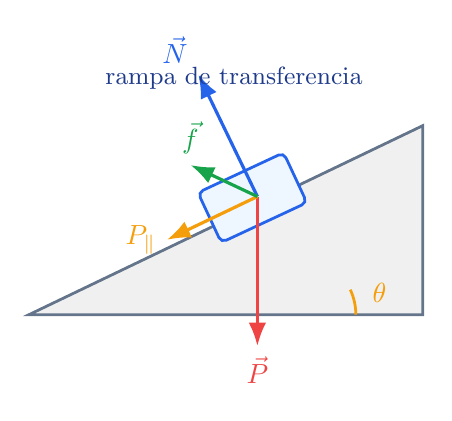
\begin{tikzpicture}[scale=1]
\coordinate (A) at (0,0); \coordinate (B) at (5,0); \coordinate (C) at (5,2.4);
\draw[fill=gray!12, draw=muted, line width=1pt] (A)--(B)--(C)--cycle;
\draw[body, rotate around={25:(2.9,1.35)}] (2.3,1.15) rectangle (3.5,1.85); \coordinate (O) at (2.9,1.5);
\draw[force,color=accentred] (O)--++(0,-1.9) node[below] {$\vec P$};
\draw[force,color=brandtwo] (O)--++(-.75,1.55) node[above left] {$\vec N$};
\draw[force,color=accentorange] (O)--++(-1.15,-.55) node[left] {$P_{\parallel}$};
\draw[force,color=accentgreen] (O)--++(-.85,.40) node[above] {$\vec f$};
\draw[accentorange,line width=1pt] (4.15,0) arc[start angle=0,end angle=25,radius=.75]; \node[text=accentorange] at (4.45,.28) {$\theta$};
\node[lab] at (2.6,3) {rampa de transferencia};
\end{tikzpicture}

\end{document}